\chapter{État de l'art}

\section*{Inroduction}
    L'assurance, aujourd'hui, est devenue un bien de consommation courante, voire de première nécessité. Il suffit de recenser les assurances dont dispose en général le simple particulier dans sa vie quotidienne : assurance auto, multirisque habitation, santé, pour les plus fréquentes, auxquelles viennent s'ajouter les assurances vie, individuelle accidents, protection juridique, loisirs... Tout le monde en conviendra, l'assurance fait partie de la vie, En d'autres termes, pas de réalisation de projet sans assurance. 
    
\section{Assurance}
    \subsection{Définition de l'assurance}
    
                
        \begin{itemize}[font=\normalsize]
                \ding{226}\textbf{ Point de vue de l’Assuré : } L’assurance est une opération par laquelle un individu (l’Assuré) se fait promettre, contre rémunération de l’assureur (la Cotisation ou prime) à son profit ou à celui d’un tiers (le Bénéficiaire) en cas de réalisation de l’aléa prévu au contrat (le Risque)
                le versement d’une prestation (l’Indemnisation)
                par l’entreprise qui propose le contrat  \\
                
                \ding{226} \textbf{ Point de vue de l’Assureur :} 
                L’assurance
correspond au fait d’utiliser l’ensemble
des
Cotisations des Assurés ,
récoltées par
l’Assureur ,
afin de pouvoir verser
l’Indemnisation
au
Bénéficiaire en cas de
réalisation du
Risque .\\
                
                
        \end{itemize}
    
    \subsection{Les types des Assurances}
 \begin{figure}[H]
\centering
\frame{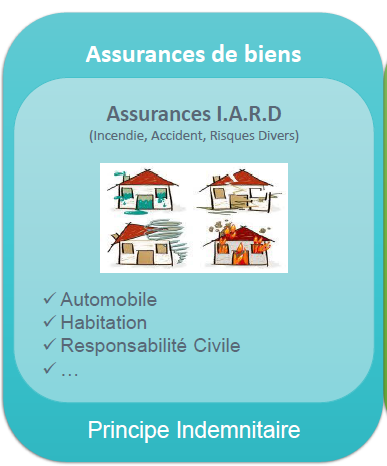
\includegraphics[width=0.5\columnwidth,height=0.4
\columnwidth]{images/Assurances_de_biens.png}}
\caption{Assurances de biens}
\label{fig:Mod-Enseig}
\end{figure}   

\begin{figure}[H]
\centering
\frame{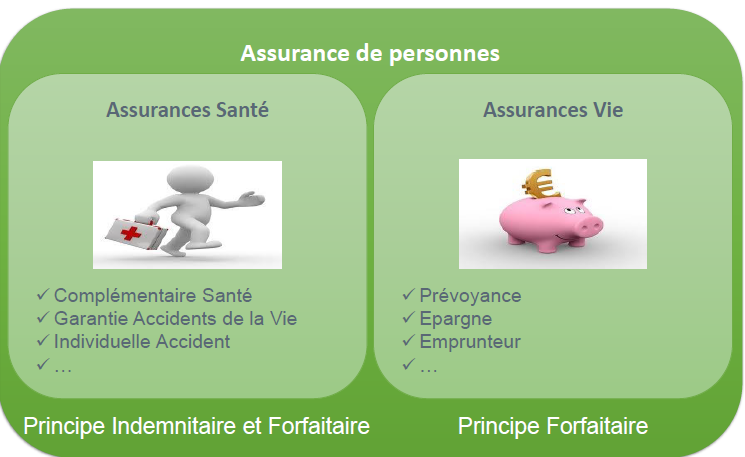
\includegraphics[width=0.5\columnwidth,height=0.4
\columnwidth]{images/Assurance_de_personnes.png}}
\caption{Assurance de personnes}
\label{fig:Mod-Enseig}
\end{figure}
\newpage
    
    \textbf{Principe Indemnitaire :}
    
    L’indemnité
due par l’assureur ne peut dépasser le
montant de la chose assurée au moment du sinistre
L’indemnité ne peut devenir une source d’enrichissement
de l’assuré
    
   
    \textbf{Principe Forfaitaire :}
    
    Le
montant du capital ou de la rente dû par l’assureur
est fixé par le contrat car le dommage subi ne peut
être évaluer objectivement.

\section{Les acteurs de l’assurance}    
    \subsection{Les Apporteurs (Réseaux de distribution)}
    \begin{figure}[H]
\centering
\frame{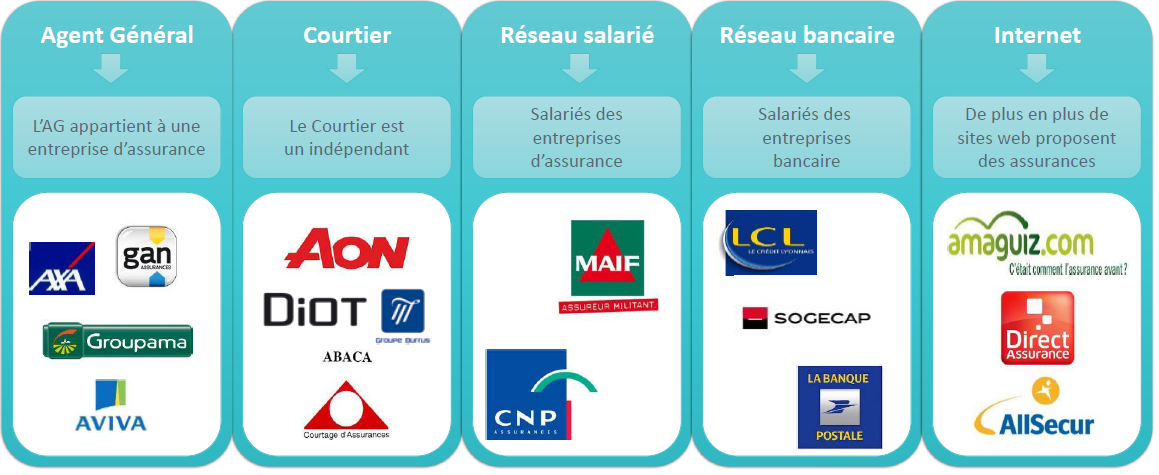
\includegraphics[width=1\columnwidth,height=0.6
\columnwidth]{images/les_acteurs_de_assurance.png}}
\caption{Les Apporteurs}
\label{fig:Mod-Enseig}
\end{figure}
       

    \subsection{Les Porteurs de Risques}
          \begin{figure}[H]
\centering
\frame{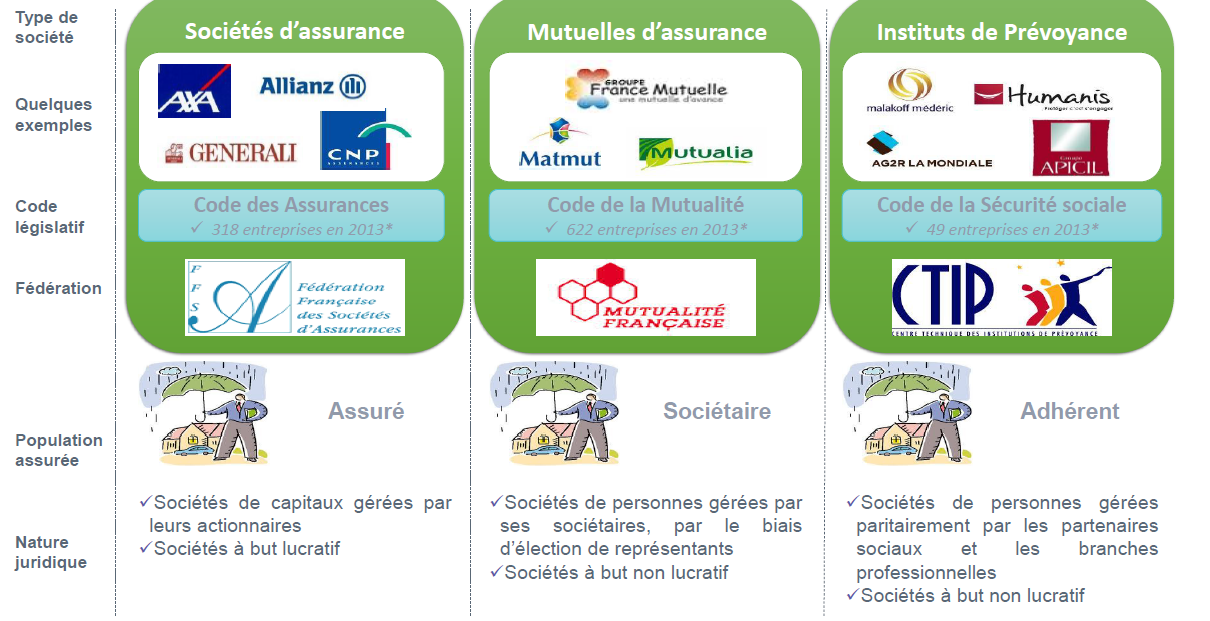
\includegraphics[width=1\columnwidth,height=0.6
\columnwidth]{images/les_porteurs_de_risques.png}}
\caption{Les porteurs de risque}
\label{fig:Mod-Enseig}
\end{figure}

          \begin{figure}[H]
\centering
\frame{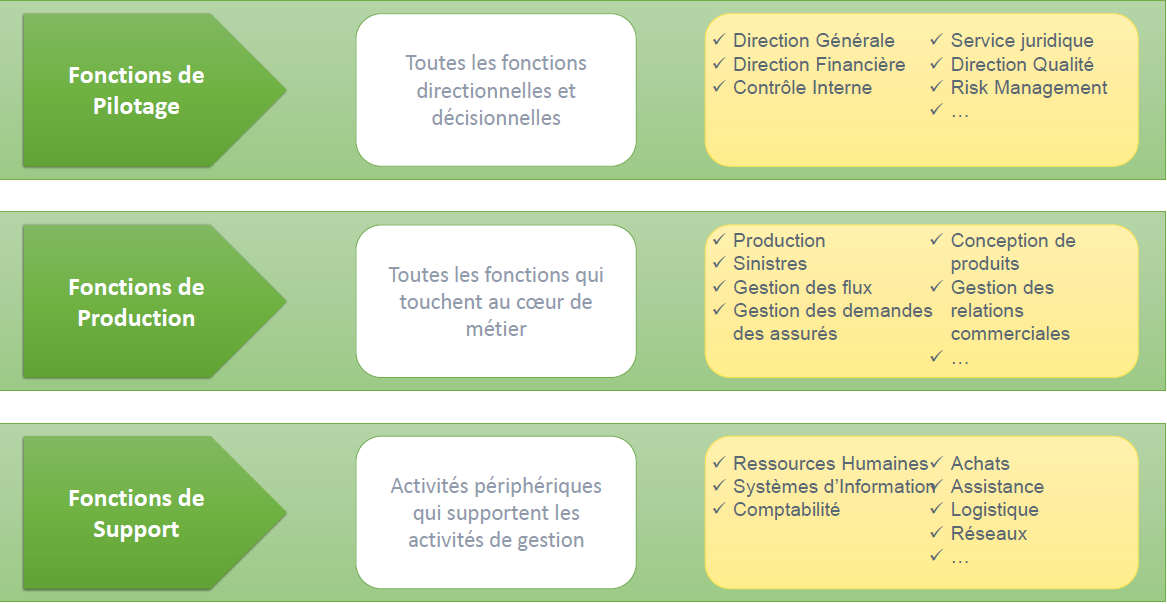
\includegraphics[width=1\columnwidth,height=0.6
\columnwidth]{images/les_porteurs_de_risques2.png}}
\caption{Les porteurs de risque}
\label{fig:Mod-Enseig}
\end{figure}
        

\newpage
    \section{Comprendre la Sécurité sociale}
    \subsection{Les 5 branches de la Sécurité sociale}
              \begin{figure}[H]
\centering
\frame{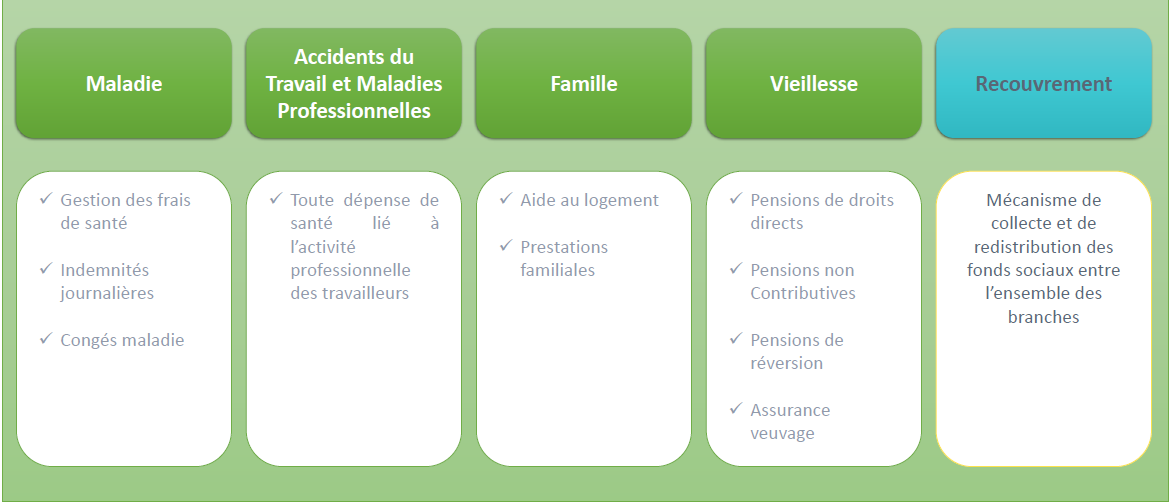
\includegraphics[width=1\columnwidth,height=0.6
\columnwidth]{images/les5.png}}
\end{figure}
    
        
        
    \subsection{Les grands régimes de la Branche Maladie}
    
    L’Assurance Maladie Obligatoire est constituée de trois principaux régimes:
    \begin{itemize}[font=\normalsize]
                \ding{226}\textbf{ Le
régime général (regroupe environ 4 personnes sur 5) }\\
\end{itemize}
\begin{itemize}[font=\normalsize]
                \ding{226}\textbf{ Le
régime des salariés agricoles }\\
\end{itemize}
\begin{itemize}[font=\normalsize]
                \ding{226}\textbf{ Le
régime social des indépendants }\\
\end{itemize}
    
    
    
               \begin{figure}[H]
                \centering
                \frame{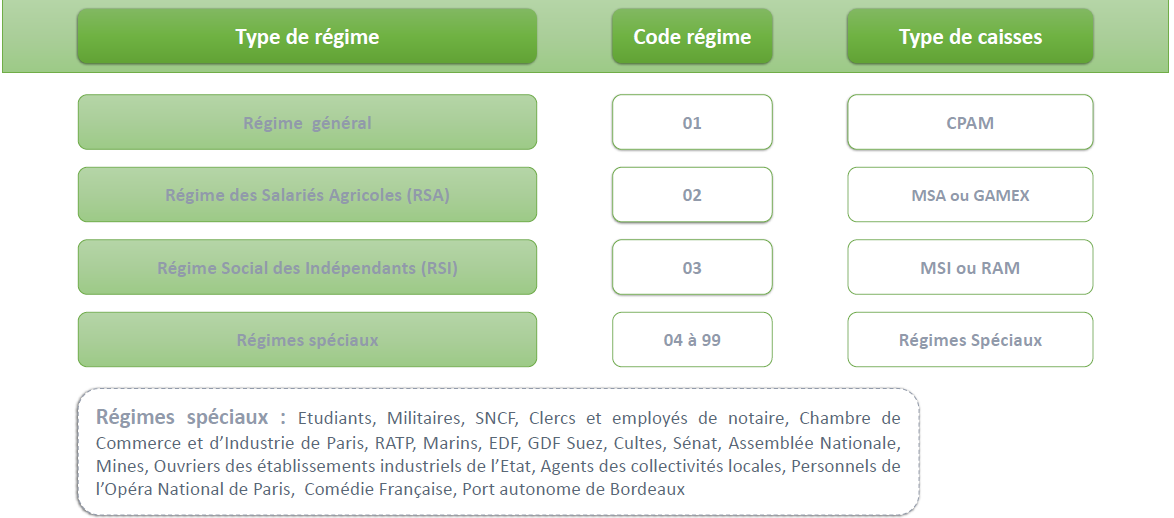
\includegraphics[width=1\columnwidth,height=0.6
                \columnwidth]{images/les6.png}}
                \end{figure}
    
        
    \subsection{Les principes de l’assurance santé}
    \begin{figure}[H]
                \centering
                \frame{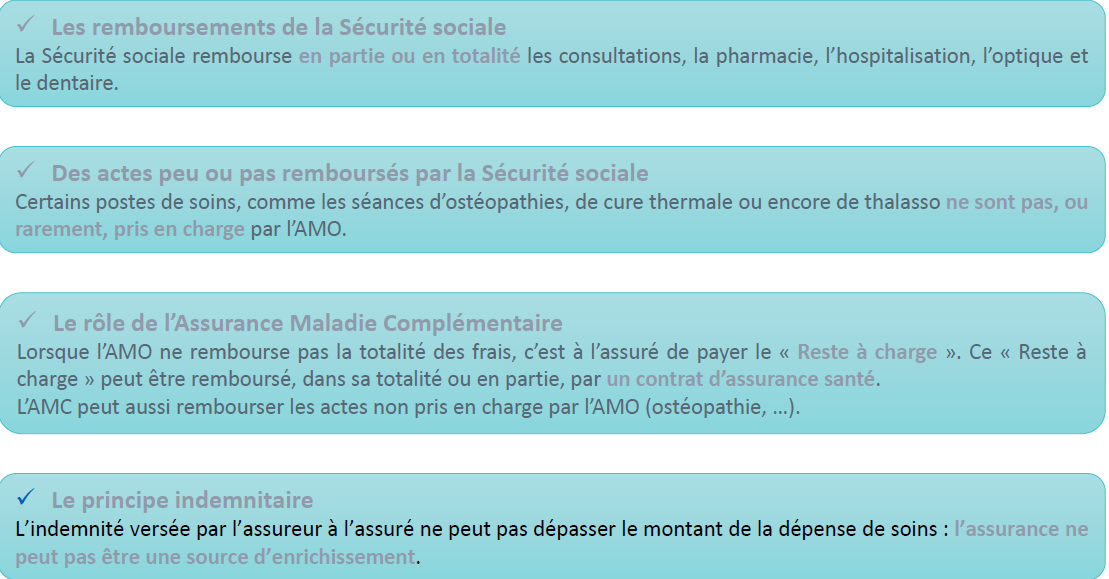
\includegraphics[width=1\columnwidth,height=0.6
                \columnwidth]{images/les7.png}}
                \end{figure}

   \section{Synthèse}
   \begin{figure}[H]
                \centering
                \frame{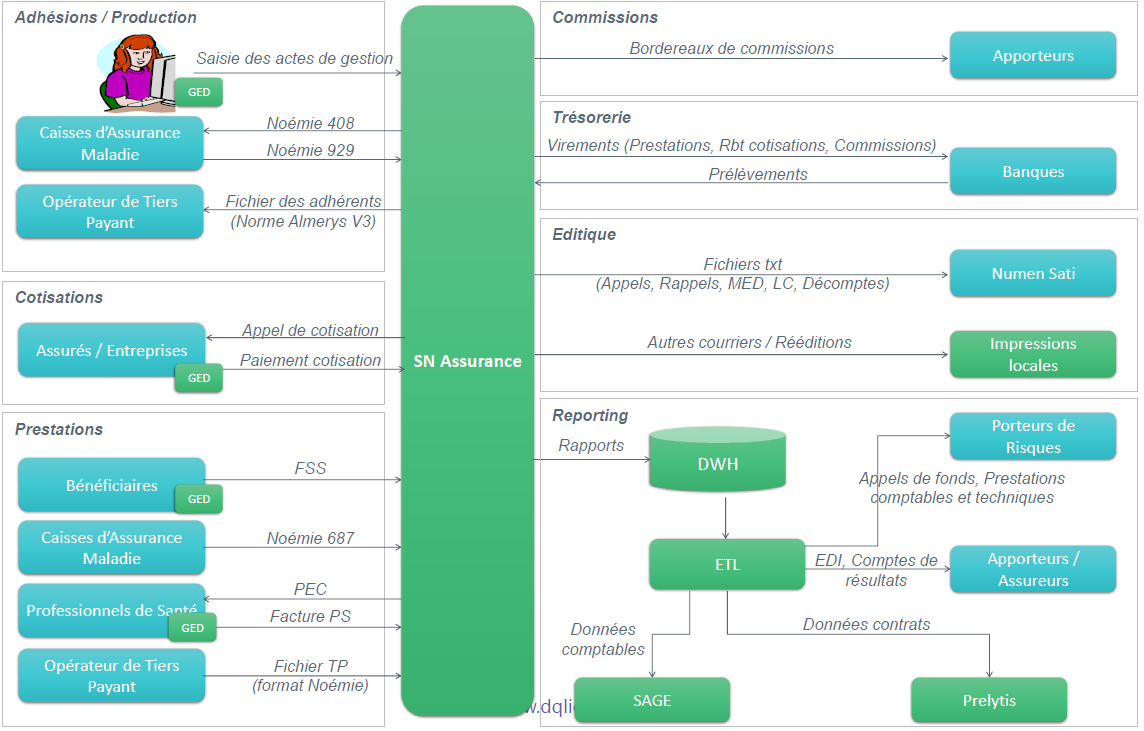
\includegraphics[width=1\columnwidth,height=0.7
                \columnwidth]{images/les8.png}}
                \end{figure}
          
    


\section*{Conclusion}
Dans ce chapitre, nous avons effectué une étude sur les différents aspects de l'assuarnce et sur les solutions existentes sur le marché national et global. Dans le chapitre suivant, nous allons dégager les besoins de nos utilisateurs en se basant sur cet étude. 